Across the 27 descriptive factorial cells, the offline policy had lower mean cost than conditional-mean MIQP in 6 cells and lower mean cost than no storage in 27 cells. The three anchors reuse complete five-restart procedures; the other 24 cells use one restart. Width contrasts therefore also reflect unequal selection effort, and the cell counts are descriptive. Realized grid exchange lay within 10 kW of the threshold for 5.77--17.31 hours/day across cells; exact-threshold occupation within $10^{-6}$ kW ranged from 5.76 to 17.31 hours/day. The corresponding mean smooth-minus-hard realized-cost difference ranged from 58.0 to 693.6 EUR/day.

\begin{figure}[t]
\centering
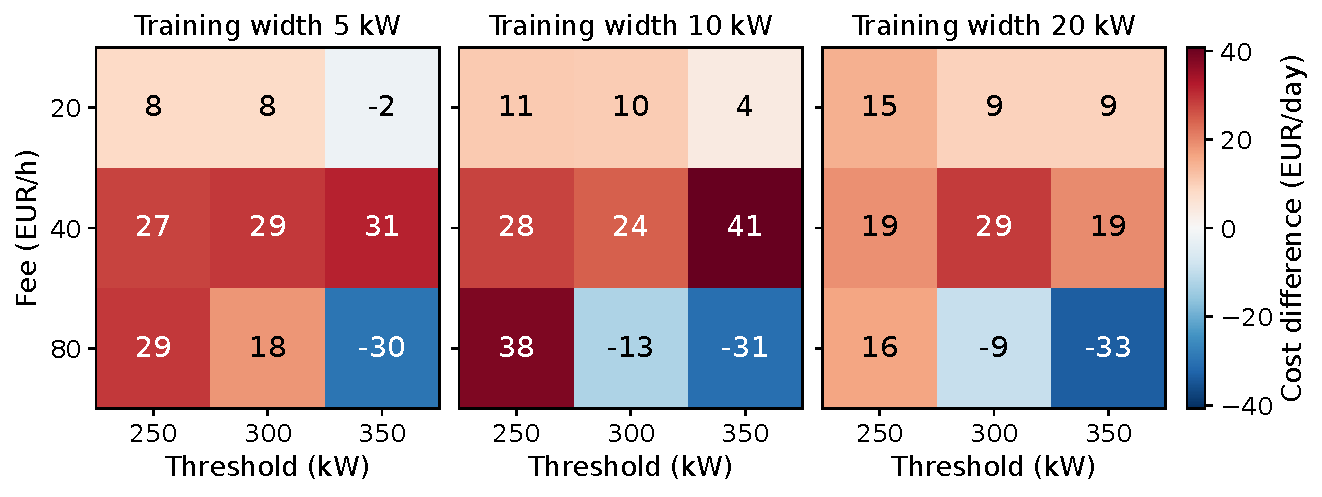
\includegraphics[width=\linewidth]{figures/fig_factorial.pdf}
\caption{Descriptive threshold--fee--smoothing results. Entries are mean offline-minus-conditional-mean-MIQP common costs in EUR/day; negative values favor the offline policy. The three anchors reuse the primary procedures; other cells use one restart.}
\label{fig:factorial}
\end{figure}